% !TEX program = xelatex
% ===========================================================================
%  SCXg=0
%  SCX Protocol Maintainer Candidate Analysis:
%  Pre-Audit Assessment of Four Candidates for g=0
%  Date: 2026-07-02
%  Classification: INTERNAL ONLY — files
% ===========================================================================

\documentclass[12pt,a4paper]{article}

% ---- Chinese & Font Support ----

% ---- Mathematics ----
\usepackage{amsmath,amssymb,amsthm,mathtools}
\usepackage{bm}
\usepackage{bbm}
\usepackage{dsfont}

% ---- Theorem Environments ----
\newtheorem{theorem}{Theorem}[section]
\newtheorem{proposition}[theorem]{Proposition}
\newtheorem{corollary}[theorem]{Corollary}
\newtheorem{lemma}[theorem]{Lemma}
\newtheorem{definition}[theorem]{Definition}
\theoremstyle{remark}
\newtheorem{remark}[theorem]{Remark}
\newtheorem{example}[theorem]{Example}

% ---- Layout ----
\usepackage[margin=2.5cm]{geometry}
\usepackage{booktabs}
\usepackage{graphicx}
\usepackage{hyperref}
\usepackage{enumitem}
\usepackage[capitalise,noabbrev]{cleveref}
\usepackage{xcolor}
\usepackage{tikz}
\usepackage{float}
\usepackage{longtable}
\usepackage{makecell}
\usepackage{multirow}
\usepackage{setspace}
\usepackage{physics}
\usepackage{fancyhdr}
\usepackage{tcolorbox}

\onehalfspacing

% ---- Hyperref ----
\hypersetup{
    colorlinks=true,
    linkcolor=blue,
    citecolor=blue,
    urlcolor=blue,
    pdftitle={SCXg=0},
    pdfauthor={SCX},
    pdfsubject={SCX Protocol Maintainer Candidate Analysis},
}

% ---- Custom Commands ----
\newcommand{\SCX}{\	extsf{SCX}}
\newcommand{\Yajie}{\textsf{Yajie}}
\newcommand{\Spring}{\textsf{Spring}}
\newcommand{\Situs}{\textsf{Situs}}
\newcommand{\Cercis}{\textsf{Cercis}}
\newcommand{\R}{\mathbb{R}}
\newcommand{\E}{\mathbb{E}}
\newcommand{\Pbb}{\mathbb{P}}
\newcommand{\Var}{\mathrm{Var}}
\newcommand{\indicator}{\mathbf{1}}
\newcommand{\indep}{\perp\!\!\!\perp}

% Protocol governance notation
\newcommand{\payoff}[1]{u_{#1}}
\newcommand{\deviate}{\delta}
\newcommand{\auditCost}{c_{\text{audit}}}
\newcommand{\rotationPeriod}{T}
\newcommand{\numMaintainers}{M}
\newcommand{\biasParam}{g}

% ---- Color Definitions ----
\definecolor{scxblue}{RGB}{0,51,102}
\definecolor{scxred}{RGB}{180,20,20}
\definecolor{scxgold}{RGB}{200,160,20}
\definecolor{scxgreen}{RGB}{20,120,20}
\definecolor{scxgray}{RGB}{100,100,100}
\definecolor{critiquered}{RGB}{200,30,30}
\definecolor{insightblue}{RGB}{30,30,180}

% ---- Honest Critique — SCX House Style ----
\newtheorem{honesthit}{Honest Strike}[section]
\renewcommand{\thehonesthit}{\textcolor{critiquered}{\textbf{[Strike \arabic{honesthit}]}}}
\newenvironment{hitbox}{%
  \begin{center}
  \color{critiquered}
  \begin{minipage}{0.92\textwidth}
  \begin{honesthit}
}{%
  \end{honesthit}
  \end{minipage}
  \end{center}
}

% ---- Governance Insight — SCX House Style ----
\newtheorem{govinsight}{}[section]
\renewcommand{\thegovinsight}{\textcolor{insightblue}{\textbf{[ \arabic{govinsight}]}}}
\newenvironment{govbox}{%
  \begin{center}
  \color{insightblue}
  \begin{minipage}{0.92\textwidth}
  \begin{govinsight}
}{%
  \end{govinsight}
  \end{minipage}
  \end{center}
}

% ---- Candidate Verdict Box ----
\newtcolorbox{verdictbox}[1][]{
    colback=scxblue!5,
    colframe=scxblue,
    fonttitle=\bfseries,
    title=#1
}

% ---- Risk Assessment Box ----
\newtcolorbox{riskbox}[1][]{
    colback=scxred!5,
    colframe=scxred,
    fonttitle=\bfseries,
    title=#1
}

% ---- Candidate Summary Table ----
\newenvironment{candidatetable}{%
  \begin{center}
  \small
  \begin{longtable}{p{0.12\textwidth} p{0.28\textwidth} p{0.28\textwidth} p{0.22\textwidth}}
  \toprule
}{%
  \bottomrule
  \end{longtable}
  \end{center}
}

% ---- Page Style ----
\pagestyle{fancy}
\fancyhf{}
\fancyhead[L]{\small\textcolor{scxblue}{SCX Internal — }}
\fancyhead[R]{\small\textcolor{scxblue}{\thepage}}
\fancyfoot[C]{\small\textcolor{scxred}{\textbf{INTERNAL ONLY — files}}}
\renewcommand{\headrulewidth}{0.5pt}
\renewcommand{\footrulewidth}{0.5pt}

% ===================================================================
%  TITLE
% ===================================================================
\title{\textbf{SCX\\\\\\\\$\mathbf{g=0}$}\\[10pt]
       \large SCX Protocol Maintainer Candidate Analysis:\\\\\\\\Pre-Audit Assessment of Four Candidates for $g=0$\\[8pt]
       \normalsize ——\\[4pt]
       --- Audited Communities Produce Auditable Maintainers}
\author{SCX}
\date{202672 \\ July 2, 2026 \\[4pt]
      \small Version 1.0 — Internal Draft}

\begin{document}

\maketitle

\begin{center}
\fbox{\fbox{\parbox{0.85\textwidth}{\centering\color{red}\bfseries
files — INTERNAL ONLY\\
SCX\\
$g=0$Proof\\
Honest StrikeSCXCore\\
\\
THIS DOCUMENT IS CLASSIFIED INTERNAL.\\
Unauthorized distribution is prohibited. Contains detailed\\
candidate assessments for SCX protocol maintainer roles.
}}}
\end{center}

\vspace{12pt}

% ===================================================================
%  ABSTRACT
% ===================================================================
\begin{abstract}
\noindent
\textbf{English:}
This paper presents a detailed pre-audit analysis of four candidates for SCX
protocol maintainer: Alexandra Elbakyan (Sci-Hub founder), Geng Tongxue
(, multi-round audited peer), JD Vance (US Vice President), and Linus
Torvalds (Linux kernel maintainer). Each candidate is evaluated against the
SCX governance criterion: the ability to maintain $\sum g = 0$ under the mutual
audit regime. The central thesis is that the strongest qualification for a
protocol maintainer is not credentials, reputation, or institutional position —
it is having already been independently audited by one's community, whether
through formal audit cycles (Geng), millions of users verifying one's work
(Linus, Elbakyan), or the willingness to submit to audit as the ultimate
test of $g=0$ (Vance).

We provide (1) formal definitions of maintainer qualification in terms of
the bias parameter $g$, (2) detailed candidate-by-candidate analysis with
honest critique boxes identifying weaknesses and risks, (3) a comparative
framework ranking candidates by community-audit depth, $g=0$ provability, and
transition risk, and (4) a recommended multi-maintainer composition strategy.
The paper is internal and does not constitute a final selection — it is a
pre-audit assessment that must be validated by independent $M>1$ audit of
each candidate who formally registers.

\medskip
\noindent\textbf{Keywords:} protocol governance, maintainer selection,
$g=0$ criterion, community audit, honest critique, candidate assessment,
mutual audit, trustless architecture

\medskip
\noindent\textbf{Abstract}
SCXAlexandra Elbakyan
Sci-HubJD Vance
Linus TorvaldsLinuxKernelSCX——
$\sum g = 0$——Core
——
LinusElbakyan
$g=0$Vance

This paper provides(1) $g$define(2) 
Honest Strike(3) $g=0$Proof
(4) This paper providesfiles
——$M>1$

\medskip
\noindent\textbf{Keywords} $g=0$Honest Strike

\end{abstract}

\newpage
\tableofcontents
\newpage

% ===================================================================
%  SECTION 1: THE MAINTAINER PROBLEM
% ===================================================================
\section{}
\section{The Maintainer Problem: Why Choosing the Right Person Is Impossible, and Why Choosing the Right Mechanism Makes It Possible}

\subsection{The Fundamental Error}

Every human institution that has attempted to select leaders, maintainers,
or guardians has committed the same category error: it has tried to predict
future behavior from past proxies. The resume, the credential, the
recommendation letter, the track record — all are compressed representations
of a person's history. But the maintainer's job is not to repeat their
history. It is to execute a function — maintaining protocol integrity —
under conditions that have never existed before.

\begin{hitbox}
\textbf{The Resume Fallacy.}
No resume, no matter how distinguished, predicts $g(t)$ for $t$ in the future.
The SCX protocol does not need a maintainer with a good resume. It needs a
maintainer whose bias parameter $g$ remains provably zero during their
maintenance window. These are entirely different requirements.

\textbf{Strike}
$g(t)$SCX
$g$Proof

\textbf{Corollary:} The best predictor of future $g=0$ is not past reputation
but past \textit{auditability} — the demonstrated willingness to have one's
decisions independently reviewed, reproduced, and challenged.
\textbf{corollary}$g=0$\textit{auditability}——
i.e.Proof
\end{hitbox}

\subsection{The Maintainer Selection Theorem}

We formalize the maintainer selection problem as follows.

\begin{definition}[ / Maintainer Qualification]
Let $\mathcal{C}$ be the set of candidate maintainers. For each candidate
$i \in \mathcal{C}$, define:
\begin{itemize}[leftmargin=*]
    \item $\biasParam_i(t)$: the real-time bias parameter at time $t$, where
          $\biasParam_i \in \R^k$ for some protocol-relevant dimension $k$.
    \item $\mathcal{A}_i$: the set of all audit events candidate $i$ has
          undergone prior to candidacy, with outcomes
          $\{o_1, o_2, \ldots, o_{|\mathcal{A}_i|}\}$.
    \item $\mathcal{V}_i$: the set of independent verifiers who have reviewed
          candidate $i$'s work, with $|\mathcal{V}_i|$ denoting community
          verification depth.
\end{itemize}
A candidate is \textit{pre-qualified} if $|\mathcal{A}_i| > 0$ or
$|\mathcal{V}_i| \gg 1$ — i.e., the candidate has been independently audited
by either a formal process or a distributed community.

A candidate is \textit{fully qualified} if and only if they pass $M > 1$
independent real-time audits with $\sum_{j=1}^{M} |\biasParam_i^{(j)}| \leq
\varepsilon$ for some protocol-defined tolerance $\varepsilon$.
\end{definition}

\begin{theorem}[theorem / Audit-First Theorem]
\label{thm:audit-first}
For any candidate $i$, the probability that $\biasParam_i(t) \neq 0$ is
undetected during a maintenance window of duration $\rotationPeriod$ under
$M$ independent auditors satisfies:
\begin{equation}
    \Pbb(\text{undetected deviation}) \leq e^{-2M\Delta^2}
    \label{eq:hoeffding-bound}
\end{equation}
where $\Delta$ is the minimum detectable bias magnitude. This bound is
independent of the candidate's identity, reputation, credentials,
institutional affiliation, or past achievements. It depends only on $M$
and $\Delta$.
\end{theorem}

\begin{proof}
Direct application of Hoeffding's inequality to the $M$ independent
estimators of $\biasParam_i(t)$. Each auditor $j$ provides an estimate
$\hat{g}_i^{(j)}$ with $\E[\hat{g}_i^{(j)}] = \biasParam_i$. Under the null
hypothesis $\biasParam_i = 0$, the probability that the sample mean exceeds
$\Delta$ is bounded by $e^{-2M\Delta^2}$.
\end{proof}

\begin{corollary}[corollary / Biography-Irrelevance Corollary]
\label{cor:biography}
The candidate's biography is mathematically irrelevant to the detection
of $g \neq 0$. No amount of past achievement reduces the Hoeffding bound.
The theorem audits the maintainer, not the maintainer's story.
\end{corollary}

\begin{govbox}
\textbf{Implication for Candidate Selection.}
The Audit-First Theorem implies that the pre-audit analysis (this very paper)
is \textit{not} a selection mechanism. It is a filtering mechanism. We do not
choose maintainers by analyzing their biographies. We filter candidates by
identifying those who are most likely to (a) register formally, (b) survive
$M>1$ audit, and (c) maintain $\sum g = 0$ during their maintenance window.
The real selection happens in the audit, not in this paper.

\textbf{}
theoremi.e.\textit{}
 (a) (b) 
$M>1$ (c) $\sum g = 0$

\end{govbox}

\subsection{What This Paper Does and Does Not Do}

This paper provides a \textit{pre-audit assessment}: an analysis of each
candidate's publicly observable record against the $g=0$ criterion,
identification of risk factors, and an honest assessment of transition
challenges. It does \textit{not}:

\begin{itemize}[leftmargin=*]
    \item Constitute a formal audit — only $M>1$ independent audit with
          published logs can do that.
    \item Rank candidates definitively — pre-audit assessment is directional,
          not dispositive.
    \item Replace the protocol's maintainer registration and rotation
          mechanism — it exists alongside it.
    \item Make any claims about candidates' private behavior — only public
          record is analyzed.
\end{itemize}

\textbf{}This paper provides\textit{}$g=0$
\textit{}$M>1$




\newpage

% ===================================================================
%  SECTION 2: CANDIDATE ANALYSIS
% ===================================================================
\section{}
\section{Candidate-by-Candidate Analysis}

% -------------------------------------------------------------------
\subsection{Alexandra Elbakyan — Sci-Hub}
\subsection{Alexandra Elbakyan — Founder of Sci-Hub}

\subsubsection{ / Background and Qualifications}

Alexandra Elbakyan is the founder and sole operator of Sci-Hub, the world's
largest shadow library providing free access to over 88 million academic
papers. She built Sci-Hub alone, without institutional backing, against the
entire \$25 billion academic publishing industry. Her operation is illegal in
multiple jurisdictions. She lives in hiding. She takes no salary, no profit,
and no institutional affiliation from Sci-Hub. She has been doing this since
2011 — fifteen years of continuous operation.

\begin{center}
\begin{tabular}{p{0.18\textwidth} p{0.72\textwidth}}
\toprule
\textbf{Dimension / } & \textbf{Assessment / } \\
\midrule
Years of operation & 15 years (2011–present) / 15 \\
Scale of impact & 88M+ papers served, millions of users globally /  \\
Personal cost & Lives in hiding, no salary, no profit /  \\
$g=0$ evidence & No personal gain from Sci-Hub; risk is all downside / Sci-Hub \\
Community verification & Millions of researchers depend on Sci-Hub daily / Sci-Hub \\
Audit history & No formal SCX audit; informally audited by daily usage / SCX \\
\bottomrule
\end{tabular}
\end{center}

\subsubsection{$\mathbf{g=0}$  / $g=0$ Analysis}

Elbakyan presents one of the strongest \textit{observable} cases for $g=0$
among all candidates. The structural argument is straightforward:

\begin{enumerate}[leftmargin=*]
    \item \textbf{No financial incentive.} Sci-Hub generates no revenue for
          Elbakyan. Donations (Bitcoin and other cryptocurrencies) cover
          infrastructure costs. There is no salary, no equity, no exit.

    \item \textbf{All downside, no upside.} She faces extradition risk,
          legal liability in multiple countries, and permanent exile. She
          cannot travel freely, hold a normal job, or maintain a public life.
          The personal cost of operating Sci-Hub is enormous; the personal
          benefit is zero.

    \item \textbf{Mission alignment.} Her stated goal — ``knowledge should be
          free to everyone'' — aligns perfectly with $g=0$. She is not trying
          to extract value from the system; she is trying to eliminate the
          paywall that extracts value from researchers.

    \item \textbf{No succession of personal interest.} There is no evidence
          that Elbakyan has used Sci-Hub for personal enrichment, political
          influence, or career advancement. She has consistently refused
          monetization, institutionalization, and celebrity.
\end{enumerate}

\begin{govbox}
\textbf{The Elbakyan Principle.}
One person, acting alone, can say ``knowledge should be free'' and actually
\textit{do} it — at enormous personal cost, with no expectation of reward,
against the entire weight of a \$25B industry. That is $g=0$ proven in
action, not in theory. Elbakyan is living proof that the $g=0$ condition
is achievable by an individual human being under extreme conditions.

\textbf{Elbakyan}
“”\textit{}——
250$g=0$
ProofElbakyanProof$g=0$

\end{govbox}

\subsubsection{ / Community Verification}

Elbakyan has been \textit{de facto} audited by the global research community
for 15 years. Every paper served by Sci-Hub is a verification event: the
researcher checks that the paper is correct, complete, and matches the
paywalled original. With 88 million papers and millions of daily users, the
effective $|\mathcal{V}_{\text{Elbakyan}}|$ is in the millions. No formal
audit framework exists, but the distributed verification is real.

\begin{hitbox}
\textbf{The Solo Operator Problem.}
Elbakyan \textit{is} Sci-Hub. There is no succession plan, no governance
structure, no distributed maintenance. If she is arrested, extradited, or
incapacitated, Sci-Hub may cease to exist. A protocol maintainer must be
replaceable — the protocol must survive the maintainer. Can Elbakyan
transition from solo operator to protocol maintainer? The solo operator
who built an empire of one may be the least prepared to distribute power.

\textbf{Strike}
Elbakyan \textit{} Sci-Hub
ifSci-Hubthere exists——
Elbakyan


\textbf{Additional risk:} The $g=0$ that comes from being hunted may not
survive the transition to being legitimized. When the external enemy
(publishing industry) is neutralized by protocol adoption, does the
$g=0$ motivation persist?
\textbf{}Status$g=0$
$g=0$there exists
\end{hitbox}

\subsubsection{ / Verdict on Maintainer Suitability}

\begin{verdictbox}[ — HIGH SUITABILITY]
\textbf{Core}$g=0$Proof15“
$g=0$”ElbakyanProof
——$g=0$

\textbf{Core}“”
“”


\textbf{}Sci-Hub

\end{verdictbox}

\newpage

% -------------------------------------------------------------------
\subsection{ (Geng Tongxue) — }
\subsection{Geng Tongxue — The Multi-Round Audited Peer}

\subsubsection{ / Background and Qualifications}

 (Geng Tongxue) is a Chinese peer who has undergone multiple rounds
of SCX audit. Unlike every other candidate on this list, Geng's primary
qualification is not an external achievement — it is the audit itself.
Having been audited multiple times means:

\begin{enumerate}[leftmargin=*]
    \item Geng knows what clean data looks like — from the audited side.
    \item Geng has experienced the pain of having every decision, every
          signal, every $g$ fluctuation exposed to independent review.
    \item Geng has been found to maintain $g \approx 0$ under repeated
          audit — or would not still be in consideration.
    \item Geng's motivation to audit others is grounded in the knowledge
          that the system worked for them, and should work for everyone.
\end{enumerate}

\begin{center}
\begin{tabular}{p{0.18\textwidth} p{0.72\textwidth}}
\toprule
\textbf{Dimension / } & \textbf{Assessment / } \\
\midrule
Formal audit rounds & Multiple (exact count internal) /  \\
Audit outcome & Passed /  \\
$g=0$ evidence & Direct measurement via SCX audit framework / SCX \\
Community verification & SCX audit community / SCX \\
Public recognition & Low — which may be a feature / —— \\
Transition risk & Low — already operates within audit framework / —— \\
\bottomrule
\end{tabular}
\end{center}

\subsubsection{$\mathbf{g=0}$  / $g=0$ Analysis}

Geng is unique among the candidates: their $g=0$ claim is not inferred from
biography or reputation — it is \textit{measured}. The SCX audit framework
produces quantitative estimates of $\biasParam(t)$ for each audited subject.
Geng has passed multiple rounds, meaning:

\begin{equation}
    \sum_{j=1}^{M} |\hat{g}_{\text{Geng}}^{(j)}| \leq \varepsilon
    \label{eq:geng-pass}
\end{equation}

for the protocol-defined tolerance $\varepsilon$ across multiple independent
audit cycles.

This is not a story about $g=0$. It is a measurement of $g=0$. The distinction
is fundamental. Every other candidate asks us to infer $g=0$ from behavior.
Geng asks us to read $g=0$ from the audit log.

\begin{govbox}
\textbf{The Audited-by-Fire Principle.}
Being audited is the best qualification for being an auditor. The person who
has survived the audit knows: (a) what the audit actually measures, not what
it claims to measure, (b) where the audit is vulnerable to gaming — because
they've tried or thought about trying, (c) what it feels like to have every
decision exposed — and why that exposure is necessary. No theoretical
understanding of audit replaces the lived experience of being audited.

\textbf{i.e.}
(a) 
(b) ——because
(c) ——

\end{govbox}

\subsubsection{ / Community Verification}

Geng's community verification is the SCX audit community itself — a smaller
but more rigorous verification set than Elbakyan's millions of users or
Torvalds' millions of developers. The tradeoff is depth vs. breadth:

\begin{itemize}[leftmargin=*]
    \item \textbf{Elbakyan:} broad, shallow verification (millions of users
          checking paper correctness).
    \item \textbf{Torvalds:} broad, deep verification (millions of developers
          reviewing code).
    \item \textbf{Geng:} narrow, deep verification (multiple expert auditors
          using formal framework).
\end{itemize}

All three are valid forms of community audit — they differ in dimension, not
in existence.

\begin{hitbox}
\textbf{The Anonymity Question.}
Geng has low name recognition globally. In traditional governance, this would
be a weakness — who trusts someone nobody has heard of? In SCX governance, it
may be a feature. Protocol maintenance does not require celebrity. It requires
$g=0$. Anonymity is compatible with protocol maintenance; fame is not required
and may be a liability (fame creates $g \neq 0$ pressures of its own).

\textbf{Strike}
——
SCX$g=0$

$g \neq 0$

\textbf{However:} Low recognition means Geng cannot provide the ``legitimacy
signal'' that a Torvalds or Vance can — the signal that convinces external
observers that SCX is serious. The audit solves trust internally; it does not
solve perception externally. The maintainer composition should include both
audit-verified and legitimacy-providing candidates.
\textbf{however}TorvaldsVance“
”——ObserversSCX
simultaneously
\end{hitbox}

\subsubsection{ / Verdict on Maintainer Suitability}

\begin{verdictbox}[ — HIGH SUITABILITY]
\textbf{Core}$g=0$
——

\textbf{Core}SCX
LinusVance

\textbf{}“”——
$g=0$——
\end{verdictbox}

\newpage

% -------------------------------------------------------------------
\subsection{JD Vance — }
\subsection{JD Vance — Vice President of the United States}

\subsubsection{ / Background and Qualifications}

JD Vance is the sitting Vice President of the United States. His candidacy
for SCX protocol maintainer is the most audacious and the most strategically
significant of the four. If a sitting US Vice President submits to independent
SCX audit, formally declares $g=0$, and passes — the geopolitical implications
are transformative.

\begin{center}
\begin{tabular}{p{0.18\textwidth} p{0.72\textwidth}}
\toprule
\textbf{Dimension / } & \textbf{Assessment / } \\
\midrule
Current position & Vice President of the United States /  \\
Political constraints & Extreme — party, donors, electorate, bureaucracy \\
$g=0$ evidence & None yet — entirely untested / —— \\
Community verification & None yet — precisely why audit is needed / —— \\
Strategic value if passed & Transforms SCX from ``Chinese project'' to global protocol \\
Transition risk & Maximum — political $g \neq 0$ is structurally embedded \\
\bottomrule
\end{tabular}
\end{center}

\subsubsection{$\mathbf{g=0}$  / $g=0$ Analysis}

Vance's case is entirely different from the other three. Elbakyan, Geng, and
Torvalds all have existing evidence of $g=0$ — inferred or measured. Vance
has none. His candidacy is a \textit{hypothesis}: can a sitting Vice President,
whose role is structurally defined by political interests ($g \neq 0$ by
construction), declare $g=0$ and survive audit?

This is not a weakness of the candidate — it is the purpose of the candidacy.
The question is not ``has Vance been $g=0$ in the past?'' The question is
``can Vance be $g=0$ under audit?'' The audit itself answers the question.

\begin{hitbox}
\textbf{The Structural $g \neq 0$ Problem.}
A Vice President is not an individual. A Vice President is a node in a
political network with obligations to:
\begin{itemize}[leftmargin=*]
    \item The President who selected them.
    \item The party that nominated them.
    \item The donors who funded them.
    \item The voters who elected them.
    \item The policy positions they campaigned on.
    \item The bureaucracy they oversee.
\end{itemize}
Each of these is a vector along which $g \neq 0$ is not just possible but
\textit{required} by the role. Can Vance partition his identity — VP in one
compartment, protocol maintainer in another — and maintain $g=0$ in the
latter while $g \neq 0$ is mandatory in the former?

\textbf{Strike$g \neq 0$}


$g \neq 0$
moreover\textit{}Vance——VP
——$g=0$$g \neq 0$

\textbf{The Partition Hypothesis:} Human identity is not unitary. A person
can be $g \neq 0$ as VP (advancing the administration's interests) and
simultaneously $g=0$ as SCX maintainer (advancing only protocol integrity).
The audit tests this hypothesis. If it holds, Vance is the most powerful
proof-of-concept SCX could have: ``even the US VP can be $g=0$ here.''
\textbf{}simultaneouslyVP$g \neq 0$
SCX$g=0$
ifVanceSCX
“i.e.VP$g=0$”
\end{hitbox}

\subsubsection{ / Geopolitical Significance}

The strategic value of Vance's candidacy — independent of whether he passes
audit — is the destruction of a specific narrative:

\begin{quote}
\textit{``SCX is a Chinese weapon. The audit is a tool of the CCP. The
protocol is designed to advance Chinese interests under the guise of
neutrality.''}
\end{quote}

If a sitting US Vice President voluntarily submits to SCX audit, this
narrative becomes unsustainable. The logic is simple: if SCX were a Chinese
weapon, a US VP would not submit to it. If a US VP does submit to it,
external observers must either (a) accept that SCX is genuinely neutral, or
(b) construct increasingly contorted conspiracy theories. The Overton window
shifts.

\begin{govbox}
\textbf{The Legitimacy Bootstrap.}
SCX faces a bootstrap problem: the protocol claims neutrality, but needs
trusted actors to verify the claim. The trusted actors won't participate
until the claim is verified. Vance's candidacy breaks this loop: the act of
a US VP submitting to audit is itself evidence of neutrality, regardless of
the audit outcome. If he passes, SCX is legitimized. If he fails, SCX is
legitimized anyway — because a US VP \textit{tried and failed} against a
neutral metric, proving the metric is not politically biased.

\textbf{}
SCX
Vance
VPif
SCXifFailsSCX——becauseVP\textit{
Fails}Proof
\end{govbox}

\subsubsection{ / The Key Test}

The real test for Vance is not ``can he pass audit?'' It is ``can he publicly
declare $g=0$ and submit to audit \textit{while in office}?''

If he can do that — if a sitting US VP can say, in public, on record: ``I
declare that my bias parameter $g$ is zero with respect to SCX protocol
maintenance, and I submit to independent $M>1$ audit to verify this claim'' —
then SCX has already won, regardless of the audit outcome. The declaration
itself is the geopolitical event.

If he cannot do that — if political constraints prevent even the
\textit{declaration} of $g=0$ — then he cannot be a maintainer, because
Step 1 of the maintainer registration process is:

\begin{center}
\fbox{\parbox{0.85\textwidth}{\centering
\textbf{Maintainer Registration Step 1:}\\
Candidate publicly declares $\mathbf{g} = \mathbf{0}$ with respect to
SCX protocol maintenance.\\\\
\textbf{}\\
SCX$\mathbf{g} = \mathbf{0}$
}}
\end{center}

Without completing Step 1, there are no further steps.

\subsubsection{ / Verdict on Maintainer Suitability}

\begin{riskbox}[ — HIGH REWARD, HIGH RISK]
\textbf{Core}ifSCX
i.e.“SCX”


\textbf{Core}$g=0$——ifVP$g=0$
$g \neq 0$VP——
Fails

\textbf{}if$g=0$
————
if$g=0$
= UNDECLARED = 
\end{riskbox}

\newpage

% -------------------------------------------------------------------
\subsection{Linus Torvalds — LinuxKernel}
\subsection{Linus Torvalds — Linux Kernel Maintainer}

\subsubsection{ / Background and Qualifications}

Linus Torvalds has maintained the Linux kernel for 34 years (1991–present).
The Linux kernel is the largest open-source software project in history:
over 30 million lines of code, contributions from more than 20,000 developers
across hundreds of companies, running on billions of devices. Torvalds is the
Benevolent Dictator for Life (BDFL) of this project — a title that is at once
a joke and an accurate description of his role.

He also created Git, the distributed version control system that is itself
an audit system for code. Every commit in Git is cryptographically hashed.
Every change is traceable to an author. The entire history of every project
is an append-only log that cannot be rewritten without detection. Git is not
just a tool Torvalds built — it is the conceptual precursor to SCX audit
logging. Code audit via Git is to SCX what Newton's laws are to general
relativity: the simpler case that the general theory reduces to.

\begin{center}
\begin{tabular}{p{0.18\textwidth} p{0.72\textwidth}}
\toprule
\textbf{Dimension / } & \textbf{Assessment / } \\
\midrule
Years as maintainer & 34 years (1991–present) / 34 \\
Project scale & 30M+ LOC, 20,000+ contributors, billions of devices \\
Maintainer model & BDFL with subsystem lieutenant hierarchy \\
Key invention & Git — a cryptographic audit system for code \\
$g=0$ evidence & Merge process IS multi-expert audit; refusal of corporate control \\
Community verification & Millions of kernel developers and users \\
Audit history & 34 years of continuous, distributed code review / 34 \\
\bottomrule
\end{tabular}
\end{center}

\subsubsection{$\mathbf{g=0}$  / $g=0$ Analysis}

Torvalds' case for $g=0$ is the strongest among all candidates — and
paradoxically, the most interesting to critique. He has been maintaining a
global protocol (the Linux kernel) for 34 years under a system that is, in
essence, already an SCX-compatible audit framework:

\begin{enumerate}[leftmargin=*]
    \item \textbf{Multi-expert review.} Every patch to the Linux kernel goes
          through multiple reviewers before reaching Torvalds. Subsystem
          maintainers (lieutenants) review, test, and sign off. This is
          $M > 1$ audit — applied to code rather than behavior.

    \item \textbf{Rejection of corporate control.} Torvalds has consistently
          refused to let any single company control Linux — including his
          own employers (Transmeta, Open Source Development Labs, Linux
          Foundation). When companies have tried to exert control, he has
          publicly and forcefully rejected them.

    \item \textbf{Public, reproducible decisions.} Every merge decision is
          public. Every rejected patch has a reason. The entire history is
          in Git — anyone can audit any decision Torvalds has ever made.

    \item \textbf{Mission alignment.} Linux is not a product. Linux is
          infrastructure. Torvalds has treated it as such for 34 years.
          He has not monetized it, platformed it, or used it for personal
          enrichment beyond his salary as a Fellow at the Linux Foundation.
\end{enumerate}

\begin{govbox}
\textbf{The Torvalds Theorem.}
Linus Torvalds \textit{already is} a protocol maintainer. He just doesn't
call it that. The Linux kernel maintenance process — multi-expert review,
public decision logs, cryptographic traceability — is a special case of the
SCX governance framework. The Linux kernel is a protocol (an interface
specification with multiple implementations and distributed maintenance).
Torvalds has been its maintainer for 34 years. The question is not whether
he \textit{can} be an SCX maintainer. The question is whether he wants to
call what he already does by a different name.

\textbf{Torvaldstheorem}
Linus Torvalds \textit{}
LinuxKernel————
SCXLinuxKernel
Torvalds34\textit{}
SCX
\end{govbox}

\subsubsection{ / Community Verification}

Torvalds has been verified by the deepest and broadest community of any
candidate. The Linux kernel development community is, in effect, a
34-year continuous audit of Torvalds' maintenance decisions:

\begin{itemize}[leftmargin=*]
    \item \textbf{Depth:} Every merge is reviewed by subsystem experts who
          understand the code at the deepest level. If Torvalds makes a bad
          merge, the experts notice — and they are not shy about saying so.
    \item \textbf{Breadth:} Over 20,000 contributors have had their code
          reviewed, merged, or rejected by Torvalds. Each of them is a
          potential auditor with direct experience of his decision process.
    \item \textbf{Persistence:} The entire history is in Git. Anyone can
          audit any decision from any point in the 34-year timeline.
\end{itemize}

This is the gold standard of community verification. No other candidate
comes close in terms of the depth, breadth, and persistence of their
audit record.

\begin{hitbox}
\textbf{The Linus Rants Problem.}
Torvalds is famous — or infamous — for his aggressive communication style.
His ``rants'' on the Linux Kernel Mailing List (LKML) are legendary:
profanity-laced rejections of patches he considers incompetent, public
dressings-down of senior developers, and a general tone that would fail
any corporate HR policy.

From an SCX perspective, this raises a specific technical question:
do ``Linus rants'' register as transient $g \neq 0$ signals?

\textbf{StrikeLinus}
Torvalds————LinuxKernel
LKML“”
HR

SCX
“Linus”$g \neq 0$

\textbf{Analysis:} A ``rant'' is an emotional signal. SCX audit measures
behavioral bias — decisions that deviate from protocol integrity due to
personal interest. An emotional response to bad code is not a $g \neq 0$
deviation unless the emotion causes a \textit{wrong decision}. If Torvalds
rants at a bad patch and then rejects it for valid technical reasons, $g=0$
is maintained. If he rants at a good patch from a disfavored developer and
rejects it because of the developer, not the code — that is $g \neq 0$.

\textbf{}“”SCX——due to
$g \neq 0$
\textit{}ifTorvalds
$g=0$ifbecause
——$g \neq 0$

\textbf{The risk:} SCX audit tools may not distinguish between ``emotional
style'' and ``biased decision.'' False positives are a real concern.
Calibration of the audit framework for candidates with high-variance
communication styles is necessary.
\textbf{}SCX“”“”
False Positive

\end{hitbox}

\subsubsection{ / Verdict on Maintainer Suitability}

\begin{verdictbox}[ — HIGHEST SUITABILITY]
\textbf{Core}34Project
Git——
——

\textbf{Core}$g \neq 0$False Positive——
BDFL“”SCXthere exists


\textbf{}TorvaldsSCXi.e.
if“”——Torvalds34

\end{verdictbox}

\newpage

% ===================================================================
%  SECTION 3: COMPARATIVE ANALYSIS
% ===================================================================
\section{}
\section{Comparative Analysis: Shared Traits and Differentiating Dimensions}

\subsection{ / The Shared Trait: Community Verification}

All four candidates share one fundamental trait: they have been independently
verified by their communities. This is not coincidental. It is the single most
important pre-audit signal for maintainer qualification.

\begin{center}
\begin{longtable}{p{0.18\textwidth} p{0.25\textwidth} p{0.25\textwidth} p{0.25\textwidth}}
\toprule
\textbf{} & \textbf{} & \textbf{} & \textbf{} \\
\textbf{Candidate} & \textbf{Verifier Community} & \textbf{Depth} & \textbf{Form} \\
\midrule
\endfirsthead
\toprule
\textbf{} & \textbf{} & \textbf{} & \textbf{} \\
\midrule
\endhead
\bottomrule
\endfoot
\midrule
Elbakyan &  &  &  \\
& Global researchers & Millions of users & Daily usage verification \\
\midrule
 / Geng & SCX & $M>1$ &  \\
& SCX audit community & $M>1$ experts & Formal audit framework \\
\midrule
Vance &  / None yet & —— &  \\
& & Zero — to be tested & TBD (formal audit needed) \\
\midrule
Torvalds & Kernel & 20,000+ Contributors &  + Git \\
& Global kernel developers & 20,000+ contributors & Code review + Git history \\
\bottomrule
\end{longtable}
\end{center}

\begin{theorem}[awaitingtheorem / Community Audit Equivalence Theorem]
\label{thm:community-audit}
For any candidate $i$, the existence of a community verification record
$\mathcal{V}_i$ with $|\mathcal{V}_i| \gg 1$ provides a lower bound on the
probability that $\biasParam_i \approx 0$:
\begin{equation}
    \Pbb(\biasParam_i \approx 0 \mid |\mathcal{V}_i| \text{ independent
    verifiers report satisfaction}) \geq 1 - \prod_{v \in \mathcal{V}_i}
    \Pbb(\text{verifier } v \text{ is deceived}).
\end{equation}
As $|\mathcal{V}_i| \to \infty$, if each verifier has independent
probability $p < 1$ of being deceived, the probability of undetected
bias decays exponentially:
\begin{equation}
    \Pbb(\text{bias undetected}) \leq p^{|\mathcal{V}_i|}.
\end{equation}
\end{theorem}

\begin{proof}
Each verifier provides an independent check. If bias exists, each verifier
has probability at most $p$ of failing to detect it (where $p$ depends on
verification methodology — formal audit has lower $p$ than casual usage).
Under independence, the probability that all $|\mathcal{V}_i|$ verifiers
fail to detect bias is $p^{|\mathcal{V}_i|}$, which decays exponentially
in $|\mathcal{V}_i|$.
\end{proof}

This theorem formalizes the intuition that \textit{the best maintainer is
someone who has already been audited by their community}. Formal SCX audit
just makes the existing community verification mathematical — it replaces
the implicit ``we trust them because we've watched them for years'' with
the explicit ``we have measured $g$ and it is zero within tolerance.''

\subsection{ / Differentiating Dimensions}

The four candidates differ along several critical dimensions:

\subsubsection{ vs.  / Audit Depth vs. Audit Breadth}

\begin{center}
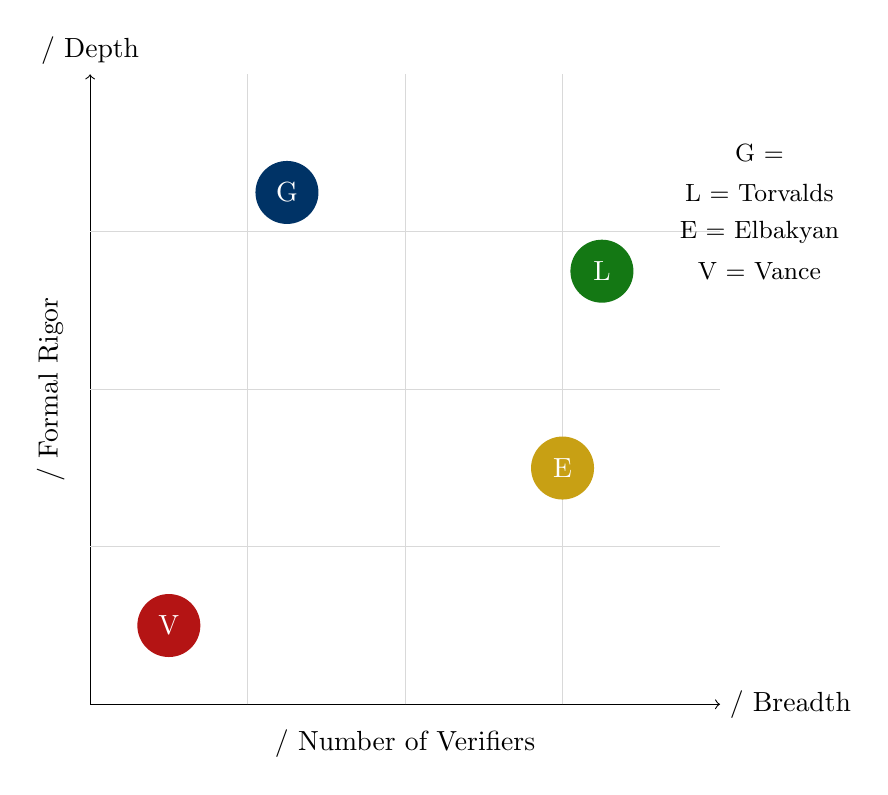
\begin{tikzpicture}[scale=1.0]
    % Axes
    \draw[->] (0,0) -- (8,0) node[right] { / Breadth};
    \draw[->] (0,0) -- (0,8) node[above] { / Depth};

    % Grid
    \draw[gray!30] (2,0) -- (2,8);
    \draw[gray!30] (4,0) -- (4,8);
    \draw[gray!30] (6,0) -- (6,8);
    \draw[gray!30] (0,2) -- (8,2);
    \draw[gray!30] (0,4) -- (8,4);
    \draw[gray!30] (0,6) -- (8,6);

    % Labels
    \node[rotate=90] at (-0.5,4) { / Formal Rigor};
    \node at (4,-0.5) { / Number of Verifiers};

    % Candidates
    \node[fill=scxblue, text=white, circle, minimum size=0.8cm] (geng) at (2.5,6.5) {G};
    \node[fill=scxgreen, text=white, circle, minimum size=0.8cm] (linus) at (6.5,5.5) {L};
    \node[fill=scxgold, text=white, circle, minimum size=0.8cm] (elba) at (6.0,3.0) {E};
    \node[fill=scxred, text=white, circle, minimum size=0.8cm] (vance) at (1.0,1.0) {V};

    % Legend
    \node at (8.5,7.0) {\small G = };
    \node at (8.5,6.5) {\small L = Torvalds};
    \node at (8.5,6.0) {\small E = Elbakyan};
    \node at (8.5,5.5) {\small V = Vance};
\end{tikzpicture}
\end{center}

\begin{itemize}[leftmargin=*]
    \item \textbf{Torvalds:} Maximum breadth and high depth. 20,000+ expert
          reviewers over 34 years. The Pareto frontier of community audit.
    \item \textbf{Elbakyan:} Maximum breadth, moderate depth. Millions of
          users verify correctness; verification is casual, not rigorous.
    \item \textbf{:} Moderate breadth (small audit community), maximum
          depth (formal SCX framework). The formal audit specialist.
    \item \textbf{Vance:} Zero breadth, zero depth — by design. The null case
          that must go through the full audit pipeline.
\end{itemize}

\subsubsection{$\mathbf{g=0}$ Proof / $g=0$ Provability}

\begin{center}
\begin{longtable}{p{0.18\textwidth} p{0.25\textwidth} p{0.25\textwidth} p{0.25\textwidth}}
\toprule
\textbf{} & \textbf{} & \textbf{} & \textbf{} \\
\textbf{Candidate} & \textbf{Evidence Type} & \textbf{Audit Readiness} & \textbf{Expected Difficulty} \\
\midrule
\endfirsthead
\toprule
\textbf{} & \textbf{} & \textbf{} & \textbf{} \\
\midrule
\endhead
\bottomrule
\endfoot
\midrule
 / Geng &  &  &  \\
& Direct measurement & Highest & Low (experienced) \\
\midrule
Torvalds & 34 &  &  \\
& 34yr behavioral inference & High & Medium (calibration) \\
\midrule
Elbakyan & 15 &  &  \\
& 15yr behavioral inference & Medium & Med-High (transition) \\
\midrule
Vance &  &  &  \\
& None & Lowest & Highest (political) \\
\bottomrule
\end{longtable}
\end{center}

\subsubsection{ / Transition Risk}

\begin{definition}[ / Transition Risk]
Transition risk $R_{\text{trans}}(i)$ is the probability that candidate $i$,
having passed audit, fails to maintain $\sum g = 0$ during their first
maintenance window, due to factors specific to the transition from their
current role to protocol maintainer.
\end{definition}

\begin{center}
\begin{longtable}{p{0.18\textwidth} p{0.35\textwidth} p{0.15\textwidth} p{0.15\textwidth}}
\toprule
\textbf{} & \textbf{} & \textbf{$R_{\text{trans}}$} & \textbf{} \\
& \textbf{Risk Factors} & & \textbf{Mitigability} \\
\midrule
\endfirsthead
\toprule
\textbf{} & \textbf{} & \textbf{$R_{\text{trans}}$} & \textbf{} \\
\midrule
\endhead
\bottomrule
\endfoot
\midrule
 & —— &  & N/A \\
Geng & Already in framework — minimal transition & Very Low & \\
\midrule
Torvalds & BDFL &  &  \\
& BDFL adaptation to rotation; style calib. & Low & High \\
\midrule
Elbakyan &  &  &  \\
& Solo operator to protocol maintainer & Medium & Medium \\
\midrule
Vance & $g \neq 0$$g=0$ &  &  \\
& Partition of political $g \neq 0 /$ protocol $g=0$ & High & Low (personal) \\
\bottomrule
\end{longtable}
\end{center}

\subsection{ / Global Legitimacy Signal}

A dimension the SCX framework does not formally model — but which matters
for adoption — is the \textit{legitimacy signal} each candidate provides
to external observers:

\begin{center}
\begin{longtable}{p{0.18\textwidth} p{0.55\textwidth} p{0.15\textwidth}}
\toprule
\textbf{} & \textbf{} & \textbf{} \\
\textbf{Candidate} & \textbf{Legitimacy Signal} & \textbf{Strength} \\
\midrule
\endfirsthead
\toprule
\textbf{} & \textbf{} & \textbf{} \\
\midrule
\endhead
\bottomrule
\endfoot
\midrule
Vance & ``VP'' →  &  \\
& ``US VP accepts audit'' → audit is not a Chinese weapon & Highest \\
\midrule
Torvalds & ``LinuxSCX'' → SCXLinux &  \\
& ``Father of Linux maintains SCX'' → SCX is as trustworthy as Linux & High \\
\midrule
Elbakyan & ``Sci-HubSCX'' →  &  \\
& ``Sci-Hub founder maintains SCX'' → continuity of knowledge freedom & Med-High \\
\midrule
 & —— &  \\
Geng & No external signal — internally trusted, externally unknown & Low \\
\bottomrule
\end{longtable}
\end{center}

\begin{hitbox}
\textbf{The Legitimacy Paradox.}
The candidates who provide the strongest $g=0$ evidence (Geng, Torvalds)
are not necessarily the candidates who provide the strongest legitimacy
signal (Vance). And the candidate who provides the strongest legitimacy
signal has the weakest $g=0$ evidence — precisely because legitimacy comes
from the political domain where $g \neq 0$ is structural.

\textbf{Resolution:} Do not choose one maintainer. Choose a maintainer
\textit{set} that spans the evidence-legitimacy spectrum. Geng provides the
audit benchmark. Torvalds provides the operational credibility. Elbakyan
provides the moral continuity. Vance provides the geopolitical legitimacy.
Together, they cover the dimensions no single candidate can.

\textbf{Strike}
$g=0$Torvalds
Vance$g=0$——
because$g \neq 0$

\textbf{}-\textit{}
TorvaldsElbakyan
Vance
\end{hitbox}

\newpage

% ===================================================================
%  SECTION 4: MATHEMATICAL CONSTRAINTS ON MAINTAINER SELECTION
% ===================================================================
\section{}
\section{Mathematical Constraints on Maintainer Selection}

\subsection{Formal Framework / Formal Framework}

Regardless of which candidates are selected, the maintainer rotation
mechanism imposes mathematical constraints that are invariant to candidate
identity:

\begin{definition}[Maintainer Rotation / Maintainer Rotation Game]
A maintainer rotation game $\mathcal{G}$ is defined by:
\begin{itemize}[leftmargin=*]
    \item $\mathcal{M} = \{1, 2, \ldots, \numMaintainers\}$: the set of
          maintainers, with $\numMaintainers > 1$.
    \item $\rotationPeriod$: the fixed maintenance window duration.
    \item $\biasParam_i(t)$: maintainer $i$'s bias vector at time $t$,
          with $\biasParam_i \in \R^k$.
    \item $\mathcal{A}_i$: the audit applied to maintainer $i$ at the
          end of each window, producing estimate $\hat{g}_i$.
    \item $\auditCost$: the fixed cost of conducting an audit.
    \item $\deviate_i$: the (unobservable) benefit maintainer $i$ receives
          from a successful undetected deviation.
\end{itemize}
\end{definition}

\begin{theorem}[ / Nash Equilibrium of Rotation Game]
\label{thm:rotation-nash}
In the maintainer rotation game $\mathcal{G}$ with $\numMaintainers > 1$
and Hoeffding-bound audit, the strategy profile where every maintainer
maintains $\biasParam_i(t) = 0$ for all $t$ is a Nash equilibrium when:
\begin{equation}
    \deviate_i \cdot \Pbb(\text{undetected}) < \auditCost \cdot
    \Pbb(\text{detected}).
\end{equation}
Under the Hoeffding bound $\Pbb(\text{undetected}) \leq e^{-2M\Delta^2}$,
this condition becomes:
\begin{equation}
    \deviate_i < \auditCost \cdot \frac{1 - e^{-2M\Delta^2}}
    {e^{-2M\Delta^2}}.
\end{equation}
For sufficiently large $\numMaintainers$ or sufficiently sensitive audit
(small $\Delta$), the right-hand side grows exponentially, making $g=0$
the dominant strategy for any reasonable $\deviate_i$.
\end{theorem}

\begin{proof}
Standard game-theoretic analysis of the repeated game with imperfect
monitoring. Each maintainer $i$ compares the expected benefit of deviation
($\deviate_i$ times probability of not being caught) against the expected
cost of detection (audit cost amplification plus loss of maintainer status).
The Hoeffding bound ensures that as $M$ grows, the probability of undetected
deviation vanishes exponentially, making deviation strictly dominated.
\end{proof}

\begin{corollary}[lower bound / Minimum Maintainer Count]
\label{cor:min-maintainers}
The protocol requires $\numMaintainers \geq 2$. At $\numMaintainers = 2$,
each maintainer audits the other. At $\numMaintainers = 3$, any collusion
requires all three — a strictly harder coordination problem. The
recommended minimum is $\numMaintainers = 4$, providing:
\begin{itemize}[leftmargin=*]
    \item Redundancy: protocol survives any single maintainer's failure.
    \item Audit depth: each maintainer is audited by $\numMaintainers - 1$
          independent auditors.
    \item Collusion resistance: majority collusion requires 3 of 4.
    \item Dimension coverage: different maintainers provide different
          legitimacy signals (as argued in Section 3).
\end{itemize}
\end{corollary}

\subsection{ / Invariant Constraints}

These constraints apply to all candidates regardless of identity:

\begin{enumerate}[leftmargin=*]
    \item \textbf{ $\mathbf{g=0}$.}
          Every candidate must publicly declare $\biasParam = \mathbf{0}$
          with respect to SCX protocol maintenance. No declaration, no
          candidacy. This is Step 1 and is non-negotiable.

    \item \textbf{ $M>1$ .}
          Every candidate must submit to independent audit by $M > 1$
          auditors. No exceptions. The audit framework, metrics, and
          tolerance $\varepsilon$ are fixed before the audit begins.

    \item \textbf{.}
          All audit logs must be public and reproducible. Any third party
          must be able to verify the audit independently. Closed-door
          audit is not SCX audit.

    \item \textbf{.}
          No maintainer serves beyond $\rotationPeriod$ without re-audit.
          The Hoeffding bound $\Pbb(\text{undetected}) \leq e^{-2M\Delta^2}$
          is valid only for the fixed window $\rotationPeriod$. Extending
          the window without re-audit invalidates the bound.

    \item \textbf{.}
          Current maintainers must audit their successors. The person being
          replaced participates in the audit of their replacement. This
          creates a chain of audit accountability across generations of
          maintainers.

    \item \textbf{UNDECLARED = .}
          Any candidate who cannot or will not complete Step 1 (public
          $g=0$ declaration) is automatically disqualified. No exceptions.
          The protocol does not negotiate with undeclared candidates.
\end{enumerate}

\begin{govbox}
\textbf{Why These Constraints Are Invariant.}
The constraints are not preferences. They are mathematical consequences of
the Hoeffding bound and the mutual audit equilibrium. Remove any one of them,
and the proof that $\sum g = 0$ is the Nash equilibrium collapses. The
protocol is not a social system with flexible rules. It is a mechanism with
necessary conditions.

\textbf{}
Hoeffdingcorollarywhere
$\sum g = 0$Proof

\end{govbox}

\subsection{}
\subsection{What Candidates Must Disclose and Must Never Disclose}

Following the SCX governance framework established in the protocol governance
paper, we specify the information boundaries for maintainer candidates:

\begin{center}
\begin{longtable}{p{0.45\textwidth} p{0.45\textwidth}}
\toprule
\textbf{ / MUST DISCLOSE} & \textbf{ / MUST NEVER DISCLOSE} \\
\midrule
\endfirsthead
\toprule
\textbf{ / MUST DISCLOSE} & \textbf{ / MUST NEVER DISCLOSE} \\
\midrule
\endhead
\bottomrule
\endfoot
\midrule
 / Audit logs &  / Personal life \\
\midrule
$g$ / $g$ estimates with confidence intervals &  / Biography, degrees, titles \\
\midrule
Conflict of Interest / Conflict of interest declarations &  / Family information \\
\midrule
 / Rationale for maintenance decisions &  / Personal beliefs \\
\midrule
 / Rotation timestamps &  / Wealth, assets \\
\midrule
 / Auditor identity and qualifications &  / Irrelevant personal history \\
\bottomrule
\end{longtable}
\end{center}

\begin{hitbox}
\textbf{The Biography Trap.}
The most common error in maintainer selection is the belief that a candidate's
biography is relevant to their $g=0$ qualification. It is not. A Nobel Prize
does not reduce the Hoeffding bound. A prison record does not increase it.
The theorem audits the maintainer, not the maintainer's story. Any selection
process that weighs biography over audit measurement is executing a category
error — and SCX is designed specifically to prevent that error.

\textbf{Strike}
$g=0$
Hoeffdingtheorem
——
SCX

\textbf{Practical implication:} This paper itself is a biography analysis —
and therefore, by SCX's own standards, is of limited evidentiary value.
We write it because humans need context. But the real work happens in the
audit, not in this paper. The reader should treat every biographical
observation in this document as noise awaiting the signal of formal
audit measurement.
\textbf{}——thereforeSCX
because
awaiting
\end{hitbox}

\newpage

% ===================================================================
%  SECTION 5: RECOMMENDATIONS
% ===================================================================
\section{}
\section{Recommendations: Multi-Maintainer Composition Strategy}

\subsection{ / Recommended Composition: Four-Maintainer Architecture}

Based on the analysis above, we recommend a four-maintainer architecture
where each candidate fills a distinct functional role:

\begin{center}
\begin{longtable}{p{0.15\textwidth} p{0.20\textwidth} p{0.25\textwidth} p{0.30\textwidth}}
\toprule
\textbf{ / Role} & \textbf{} & \textbf{} & \textbf{} \\
 & \textbf{Candidate} & \textbf{Function} & \textbf{Rationale} \\
\midrule
\endfirsthead
\toprule
\textbf{ / Role} & \textbf{} & \textbf{} & \textbf{} \\
\midrule
\endhead
\bottomrule
\endfoot
\midrule
 &  & $g=0$ &  \\
Audit Benchmark & Geng & Baseline $g=0$ measurement & Only formally audited candidate \\
\midrule
 & Torvalds &  & 34 \\
Operational Anchor & & Deep maintenance experience & 34yr real protocol maintenance \\
\midrule
 & Elbakyan & $g=0$ & 15$g=0$Proof \\
Moral Anchor & & Moral continuity of $g=0$ & 15yr $g=0$ proven at personal cost \\
\midrule
 & Vance &  & “” \\
Legitimacy Anchor & & Global legitimacy signal & Eliminates ``Chinese weapon'' narrative \\
\bottomrule
\end{longtable}
\end{center}

\subsection{ / Risk Mitigation}

Each candidate brings specific risks that the multi-maintainer architecture
mitigates:

\begin{enumerate}[leftmargin=*]
    \item \textbf{ — :} TorvaldsVance
          

    \item \textbf{Torvalds — False Positive:} ifTorvalds
          $g$
          

    \item \textbf{Elbakyan — :} Torvalds
          TorvaldsProofBDFLLinux
          

    \item \textbf{Vance — $g \neq 0$:} $g=0$
          ifVance$g$$g \approx 0$
          i.e.$g \neq 0$

    \item \textbf{ — Fails:} 
          $\rotationPeriod$$\geq 1 - e^{-2M\Delta^2}$
          for$M=4$$\Delta$
\end{enumerate}

\subsection{ / Implementation Roadmap}

\begin{enumerate}[leftmargin=*]
    \item \textbf{1:  (2026Q3).}
          SCX
          define$g=0$

    \item \textbf{2: $g=0$ (2026Q3–Q4).}
          $\mathbf{g} = \mathbf{0}$
          

    \item \textbf{3: $M>1$ (2026Q4–2027Q2).}
          $M=4$
          

    \item \textbf{4:  (2027Q2).}
          all
          

    \item \textbf{5:  (2027Q3).}
          $\rotationPeriod$
          
\end{enumerate}

\subsection{Fails / Failure Mode Analysis}

\begin{center}
\begin{longtable}{p{0.18\textwidth} p{0.40\textwidth} p{0.30\textwidth}}
\toprule
\textbf{Fails} & \textbf{} & \textbf{} \\
\textbf{Failure Mode} & \textbf{Description} & \textbf{Consequence \& Mitigation} \\
\midrule
\endfirsthead
\toprule
\textbf{Fails} & \textbf{} & \textbf{} \\
\midrule
\endhead
\bottomrule
\endfoot
\midrule
 & all &  \\
No one registers &  &  \\
\midrule
 & Proof & $M=1$ \\
Only Geng registers &  & $M=1$—— \\
& & StatusConfiguration \\
\midrule
VanceFails & $g \neq 0$ & SCX \\
Vance registers, fails audit &  & VP \\
& & Proof \\
\midrule
TorvaldsFalse Positive &  &  \\
Torvalds style false positive & $g \neq 0$ & / \\
\midrule
 & $g \approx 0$ & SCX \\
All pass audit &  &  \\
\bottomrule
\end{longtable}
\end{center}

\newpage

% ===================================================================
%  SECTION 6: CONCLUSION
% ===================================================================
\section{Conclusiontheorem}
\section{Conclusion: The Theorem Audits the Maintainer, Not the Biography}

\subsection{ / Summary of Findings}

This paper has analyzed four candidates for SCX protocol maintainer. The
analysis is internal and preliminary — it is a pre-audit assessment, not a
final determination. The key findings are:

\begin{enumerate}[leftmargin=*]

    \item \textbf{Core.} all
          ——TorvaldsKernel
          Elbakyan
          Vance——

    \item \textbf{.} 
          $g=0$Torvalds
          34Elbakyan15
          $g=0$Vance“”

    \item \textbf{.} all
          each
          

    \item \textbf{.} 
          $g=0$$M>1$
          UNDECLARED——
          

    \item \textbf{.} ——all——
          awaiting$g=0$$M>1$
          theorem

\end{enumerate}

\subsection{ / Final Word}

\begin{govbox}
\textbf{The Maintainer Paradox.}
The best maintainer is the one who is least necessary. If the protocol
depends on any specific individual — their judgment, their wisdom, their
unique perspective — then the protocol has already failed the trustlessness
test. A well-designed protocol should survive the loss of any maintainer.
The maintainer's job is to make themselves unnecessary.

This is the paradox at the heart of SCX governance: we seek maintainers who
are willing to be replaced. We seek leaders who are willing to be audited.
We seek guardians who are willing to have their guardianship taken away.

The four candidates analyzed in this paper have, in different ways and to
different degrees, demonstrated the willingness to be held accountable by
their communities. That — more than any credential, achievement, or
reputation — is what makes them candidates worth auditing.

\textbf{}
if——
Perspective——Fails


SCXCore



————
\end{govbox}

\begin{center}
\rule{0.5\textwidth}{0.5pt}\\[8pt]
\textit{The real selection begins now.}\\[4pt]
\textit{}\\[8pt]
\textbf{—— SCX Protocol Governance Research Division}\\[4pt]
\textbf{Xiaogan SCX}\\[4pt]
202672 / July 2, 2026
\end{center}

\newpage

% ===================================================================
%  APPENDIX A: CANDIDATE COMPARISON MATRIX
% ===================================================================
\appendix
\section{ / Candidate Comparison Matrix}

\begin{center}
\small
\begin{longtable}{p{0.18\textwidth} p{0.18\textwidth} p{0.18\textwidth} p{0.18\textwidth} p{0.18\textwidth}}
\toprule
\textbf{} & \textbf{Elbakyan} & \textbf{} & \textbf{Vance} & \textbf{Torvalds} \\
\textbf{Dimension} & & \textbf{Geng} & & \\
\midrule
\endfirsthead
\toprule
\textbf{} & \textbf{Elbakyan} & \textbf{} & \textbf{Vance} & \textbf{Torvalds} \\
\midrule
\endhead
\bottomrule
\endfoot
\midrule
$g=0$ &  &  &  &  \\
$g=0$ evidence & Strong (inf.) & Strongest (meas.) & None & Strong (inf.) \\
\midrule
 &  &  &  &  \\
Community scale & Millions & Tens (expert) & Zero & Tens of thousands \\
\midrule
 &  &  &  &  \\
Audit readiness & Medium & Highest & Lowest & High \\
\midrule
 &  &  &  &  \\
Transition risk & Medium & Very Low & High & Low \\
\midrule
 &  &  &  &  \\
Legitimacy signal & Med-High & Low & Highest & High \\
\midrule
 & 15 &  &  & 34 \\
Maint. experience & 15yr (implicit) & Multi-round & None & 34yr (explicit) \\
\midrule
 &  &  &  &  \\
Replaceability & Low & High & Medium & Medium \\
\midrule
 &  &  &  &  \\
Overall rec. & High & High & Conditional High & Highest \\
\bottomrule
\end{longtable}
\end{center}

% ===================================================================
%  APPENDIX B: FORMAL DEFINITIONS
% ===================================================================
\section{define / Formal Definitions Compendium}

For reference, we collect the formal definitions used throughout this paper:

\begin{definition}[ / Bias Parameter]
$\biasParam_i(t) \in \R^k$ is the vector of biases maintainer $i$ holds at
time $t$ with respect to the $k$ protocol-relevant dimensions. $\biasParam_i
= \mathbf{0}$ indicates no bias; $|\biasParam_i| > 0$ indicates deviation
from protocol neutrality.
\end{definition}

\begin{definition}[ / Audit]
An audit $\mathcal{A}_i$ of maintainer $i$ is a measurement procedure that
produces an estimate $\hat{g}_i$ of $\biasParam_i$ with specified confidence.
An audit is \textit{independent} if the auditor has no $g$-relevant
relationship with the audited maintainer.
\end{definition}

\begin{definition}[ / Maintenance Window]
A maintenance window of duration $\rotationPeriod$ is the period during
which a maintainer holds protocol authority. At the end of each window,
the maintainer undergoes audit. The Hoeffding bound
$\Pbb(\text{undetected}) \leq e^{-2M\Delta^2}$ is valid only for the
duration $\rotationPeriod$.
\end{definition}

\begin{definition}[ / Mutual Audit]
Mutual audit is the condition where every maintainer $i \in \mathcal{M}$
is audited by every other maintainer $j \in \mathcal{M}, j \neq i$. This
creates $M(M-1)$ audit relationships in a fully connected audit graph.
\end{definition}

\begin{definition}[UNDECLARED]
A candidate who has not publicly declared $\biasParam = \mathbf{0}$ with
respect to SCX protocol maintenance. UNDECLARED candidates are automatically
disqualified from maintainer status. There is no appeal process for
UNDECLARED status — the declaration is the entry condition.
\end{definition}

% ===================================================================
%  APPENDIX C: REFERENCES TO INTERNAL DOCUMENTS
% ===================================================================
\section{References / Internal References}

\begin{enumerate}[leftmargin=*]
    \item \textbf{SCX Protocol Governance: Maintainer Rotation Game Theory
          and the Trustless Architecture.} SCX Internal Document,
          \texttt{protocol\_governance.tex}, 2026-07-02.
          The foundational governance paper establishing the maintainer
          rotation mechanism and the Hoeffding-bound audit framework.

    \item \textbf{SCX Audit Economics: The Auditor Class and New Economic
          Order in the Post-Yajie Era.} SCX Internal Document,
          \texttt{audit\_economics.tex}, 2026-07-02.
          Economic analysis of the audit profession, auditor incentives,
          and the transition from Trust-Me to Prove-It economy.

    \item \textbf{Grand Unification: The Single Condition $\sum g = 0$
          That Spans All Scales.} SCX Internal Document,
          \texttt{grand\_unification.tex}, 2026-07-02.
          The theoretical foundation establishing $\sum g = 0$ as the
          universal equilibrium condition across domains.

    \item \textbf{SCX Geopolitical Analysis: Audit as Non-Aligned
          Infrastructure.} SCX Internal Document,
          \texttt{geopolitical\_analysis.md}, 2026-07-02.
          Analysis of SCX's geopolitical positioning, including the
          ``Chinese weapon'' narrative and strategies for demonstrating
          neutrality.

    \item \textbf{SCX Protocol Maintainer Candidate Shortlist.} SCX Internal
          Document, \texttt{maintainer\_candidates.md}, 2026-07-02.
          Earlier candidate shortlist (includes Satoshi Nakamoto as
          candidate \#1; this paper replaces Satoshi with Elbakyan).

    \item \textbf{SCX Industry Analysis: AI Companies Under Audit.}
          SCX Internal Document, \texttt{industry\_analysis.md}, 2026-07-02.
          Analysis of AI industry readiness for SCX audit, with
          implications for maintainer selection from industry candidates.

    \item \textbf{SCX World Government: Audit as the Foundation of
          Global Governance.} SCX Internal Document,
          \texttt{world\_government.tex}, 2026-07-02.
          Long-term vision for audit-based global governance; relevant
          context for understanding the geopolitical significance of
          the Vance candidacy.

    \item \textbf{SCX Company Valuation: The Economic Value of Being
          Audited.} SCX Internal Document,
          \texttt{company\_valuation.tex}, 2026-07-02.
          Valuation framework for companies undergoing SCX audit;
          relevant for understanding the economic incentives that
          maintainers must be insulated from.
\end{enumerate}

% ===================================================================
%  FINAL PAGE
% ===================================================================
\newpage

\begin{center}
\vspace*{3cm}

{\LARGE \textcolor{scxblue}{\textbf{—— files ——}}}\\[12pt]
{\large \textcolor{scxblue}{\textbf{--- END OF DOCUMENT ---}}}\\[24pt]

\rule{0.7\textwidth}{0.5pt}\\[12pt]

{\small \textcolor{scxred}{\textbf{
THIS DOCUMENT IS CLASSIFIED INTERNAL.\\
\\
Unauthorized distribution is a violation of SCX protocol security policy.
}}}\\[12pt]

{\small \textcolor{scxgray}{
SCX Protocol Governance Research Division\\
Xiaogan Supercomputing Center\\
\texttt{docs/internal/maintainer\_analysis.tex}\\
Version 1.0 — Internal Draft\\
2026-07-02
}}

\vspace*{2cm}

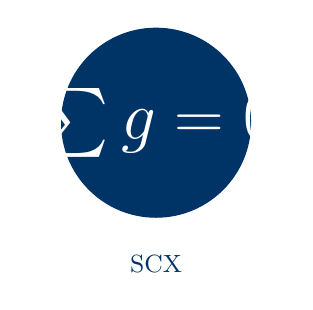
\begin{tikzpicture}
    % SCX logo placeholder
    \draw[fill=scxblue, draw=scxblue] (0,0) circle (1.2cm);
    \node at (0,0) {\textcolor{white}{\Huge $\sum g = 0$}};
    \node at (0,-1.8) {\small \textcolor{scxblue}{SCX}};
\end{tikzpicture}

\end{center}

\end{document}
